\RequirePackage{etex} 
\documentclass[xcolor=svgnames]{beamer}
%
\usetheme{Singapore}
\setbeamertemplate{navigation symbols}{}
\setbeamertemplate{footline}[frame number]

%
\setbeamercolor{block body}{bg=AliceBlue}

\usepackage[all]{xy}
\usepackage{accents}
\usepackage{amsmath,amssymb}
\usepackage{array}
\usepackage{bibentry}
\usepackage{bm}
\usepackage{cancel}
\usepackage{comment}
%\usepackage{etex}
\usepackage{macros}
\usepackage{mathscinet}
\usepackage{mathtools}
\usepackage{rotating}
\usepackage{tikz}

\hypersetup{
    colorlinks=true,
    linkcolor=blue,
    filecolor=magenta,      
    urlcolor=cyan
    }
\renewcommand{\newblock}{\relax} %% ??????????

%
%% Gianni macros
%

\DeclareMathOperator{\Hajek}{Hajek}
\DeclareMathOperator{\M}{\mathcal M}
\DeclareMathOperator{\eDeriv}{D_{\text{e}}}
\DeclareMathOperator{\grad}{grad}
\DeclareMathOperator{\mDeriv}{D_{\text{m}}}

\newcommand{\Bspaceat}[1]{B_{#1}}
\newcommand{\Bspace}[1]{B_{#1}}
\newcommand{\Ccs}[1]{C_0\left(#1\right)}
\newcommand{\Cexp}[1]{C_0^{(\cosh-1)}\left(#1\right)}
\newcommand{\Cinfcs}[1]{C_0^\infty\left(#1\right)}
\newcommand{\Cinfp}[1]{C_{\mathrm{p}}^\infty\left(#1\right)}
\newcommand{\Derivby}[1]{\frac{\Deriv}{d#1}}
\newcommand{\Lexp}[1]{L^{(\cosh-1)}\left(#1\right)}
\newcommand{\LlogL}[1]{L^{(\cosh-1)_*}\left(#1\right)}
\newcommand{\TMaxexp}{\operatorname{T}\Maxexp}
\newcommand{\WCexp}[1]{C_0^{1,(\cosh-1)}\left( #1 \right)}
\newcommand{\Wexp}[1]{W^{1,(\cosh-1)}\left(#1\right)}
\newcommand{\WlogL}[1]{W^{1,(\cosh-1)_*}\left(#1\right)}
\newcommand{\bgamma}{{\bm \gamma}}
\newcommand{\bnabla}{{\bm\nabla}}
\newcommand{\condexpectat}[3]{{\Expectation}_{#1}\left[#2 \middle| #3\right]}
\newcommand{\displacement}{\operatorname{\mathbb S}}
\newcommand{\eBspace}[1]{B_{#1}}
\newcommand{\eDerivby}[1]{\frac{\eDeriv}{d#1}}
\newcommand{\ehessianat}[2]{\prescript{e}{}\Hessian_{#1}{#2}}
\newcommand{\expbundle}{S\Maxexp}
\newcommand{\fullbundleat}[1]{\prescript{1}{}S^1\maxexpat{#1}}
\newcommand{\gaussdensity}{\gamma}
\newcommand{\gaussint}[2]{\int{#1} \gaussdensity(#2) \ d#2 \ }
\newcommand{\hajekof}[1]{\Hajek\left(#1\right)}
\newcommand{\hullof}[1]{\operatorname{hull}\left(#1\right)}
\newcommand{\mDerivby}[1]{\frac{\mDeriv}{d#1}}
\newcommand{\maxmix}[1]{\prescript{*}{}{\Maxexp\left(#1\right)}}
\newcommand{\mhessianat}[2]{\prescript{m}{}\Hessian_{#1}{#2}}
\newcommand{\mixbundleat}[1]{\prescript{*}{}S\maxexpat{#1}}
\newcommand{\mixbundle}{\prescript{*}{}S\Maxexp}
\newcommand{\mixfiberat}[2]{{}^*S_{#1}\maxexpat{#2}}
\newcommand{\model}{\mathcal M}
\newcommand{\openplan}[2]{\overset{\circ}\Pi\left(#1,#2\right)}
\newcommand{\opensimplexat}[1]{\mathcal P_>\left(#1\right)}
\newcommand{\preBspaceat}[1]{\prescript{*}{}B_{#1}}
\newcommand{\preBspace}[1]{\prescript{*}{}B_{#1}}
\newcommand{\rosso}[1]{\textcolor{red}{#1}}
\newcommand{\sdomainat}[1]{\sdomain_{#1}}
\newcommand{\sdomain}{\mathcal S}
\newcommand{\simplexon}[1]{\mathcal P\left(#1\right)}
\newcommand{\tensorat}[3]{\prescript{#1}{}S^{#2}\maxexpat{#3}}
\newcommand{\opensimplexon}[1]{\mathcal P_>\left(#1\right)}

\renewcommand{\emph}{\rosso}
\renewcommand{\transport}[2]{{\mathbb U} _ {#1} ^ {#2}}

%
%% end Gianni's macros
%

\title{B0262 \\ \it Information geometry of ANOVA and transport on a finite state space}

\author[G Pistone]{Giovanni Pistone}

\institute[CCA]{
\includegraphics[height=4em]{pictures/deCastro-logo.pdf}}
  
\date{Compiled \today}

\begin{document} 
% 
\begin{frame}\frametitle{EO357 CMStatistics 2023 }  

\titlepage

\tiny 
web-page: \url{www.giannidiorestino.it} 

e-mail: \url{giovanni.pistone@carloalberto.org}

orcidID: 0000-0003-2841-788X

The author acknowledges the support of de Castro Statistics and  INdAM-GNAMPA.

\nobibliography{tutto}%

\bibliographystyle{plain}

\end{frame}

\begin{frame}[plain]\small\frametitle{Abstract}

\emph{Functional ANOVA} (Analysis of variance) appears in Statistics and System Theory. It is a particular orthogonal splitting of the vector space of square-integrable random variables on a product space. When the sample space is factorial,  it conveniently splits the fibres of the \emph{affine bundle} consisting of couples of probability functions and Fisher's scores, which we call the \emph{Statistical Bundle}. One of the terms in the splitting is the \emph{additive model}, while the other is related to the \emph{transportation model} with fixed margins. This concept is known in the classical theory of contingency tables. We rephrase it and show implications to algebraic statistics, information geometry, and Kantorovich optimal transport. In this setting, the \emph{gradient flow} in the transport sub-model has a limit point that solves the \emph{Kantorovich problem}.

\end{frame}

\begin{frame}[plain]\small\frametitle{References}
\tiny 

\begin{description}
    \item[1968] \bibentry{hajek:1968}
    \item[1981] \bibentry{efron|stein:1981variance}
    \item[2001] \bibentry{sobol:2001global}
    \item[2021] \bibentry{pistone:2021gsi}
    \item[2021] \bibentry{pistone|rapallo|rogantin:2021}
    \item[2022] \bibentry{chirco|pistone:2022}
\end{description}
\end{frame}

\begin{frame}

\huge PART 1: KEYWORDS EXPLAINED
    
\end{frame}

    \begin{frame}[plain,allowframebreaks]\small\frametitle{ANOVA with two non-independent factors}

    \begin{itemize}
    \item Consider a finite product sample space $\Omega = \Omega_1 \times \Omega_2$. The generic probability function is denoted
    \begin{equation*}
       q \colon  \Omega_1 \times \Omega _2 \ni (x_1,x_2) \mapsto q(x_1,x_2) \ . 
    \end{equation*}
    We denote the two margins by 
    \begin{equation*}
    q_1(x_1) = \sum_y f(x_1,y) \ , \quad q_2(x_2) = \sum_x q(x,x_2) \ .
    \end{equation*}
    \item Occasionally, we use a numbering $\Omega_k = \set{1,\dots,n_k}$ and identify $q$ with a matrix $Q \in \reals^{n_1 \times n_2}$.
    \item For each random variable $f \in L^2(q)$ we look for an orthogonal decomposition of the form
    \begin{equation*}
        f(x_1,x_2) = f_0 \oplus (f_1(x) + f_2(x_2)) \oplus f_{12}(x_1,x_2)
    \end{equation*}
    \item Notice that we do not require $f_1 \perp f_2$ as it is done in case of independence, cf Hajek:1968 and Sobol':2001.
    \item We call \emph{factors} the two projections \begin{equation*}
    X_1 \colon (x_1,x_2) \mapsto x_1 \ , \quad X_2 \colon (x_1,x_2) \mapsto x_2 \ .  
    \end{equation*}
  \item Consider the subsets $I \subset \set{1,2}$, partially ordered by inclusion, that is, 
\begin{equation*}\emptyset \prec \set{1},\set{2} \prec \set{1,2} \ .
\end{equation*}
\item  Each $I \neq \emptyset$ is an \emph{interaction}. 
   Let $X_I$ be the components projection on $I$, $X_I = (X_j \colon j \in I)$.
    \item A $q$-effect is a random variable with zero $Q$-mean. A \emph{$q$-effect of the interaction $I$} is a $q$-effect of the form $f\circ X_I$ which is $q$-orthogonal to all $g \circ X_J$ for all $J \prec I$, that is, $J \subset I$ and $J \neq I$.
    \item The \emph{order} of the interaction $I$ is $\# I$. Let $H_k$ be the vector space generated by the $I$-interactions of order $k$. $H_0$ contains random variables which do not depend on any $X_j$ $j=1,2$. that is, $H_0 = \reals$.
    \item The space $H_1$ is generated by the random variables of the form 
        $f_1\circ X_1$ and $f_2\circ X_2$
    with 
    \begin{gather*}
        \expectat q {f_1\circ X_1} = \expectat {q_1} {f_1} = 0 \\
           \expectat q {f_2\circ X_2} = \expectat {q_2} {f_2} = 0 
    \end{gather*}
   \item An element of $H_1$ is of the form
   \begin{equation*}
       f_1\circ X_1 + f_2 \circ X_2 \ , \quad f_1 \in L^2_0(q_1) \ , f_2 \in L^2_0(q_2)
   \end{equation*}
   \item The representation above is unique. In fact, if
   \begin{equation*}
       f_1(x_1) + f_2(x_2) = 0 \ , x_1 \in \Omega_1, x_2 \in \Omega_2 \ ,
   \end{equation*}
   then both $f_1$ and $f_2$ must be constant. As the $q$-expectation is zero, $f_1 = f_2 = 0$.
   \item An element of $H_2$ is of the form $f_{12} \circ(X_1,X_2)$ with
   \begin{equation*}
     f_{12} \circ(X_1,X_2) \perp H_{\emptyset}, H_{\set{1}}, H_{\set{2}}  
   \end{equation*}
   The orthogonality with respect to $H_{\emptyset}$ implies zero $q$-expectation $\expectat q {f_{12}} = 0$. The orthogonality with respect to $H_{\emptyset} + H_{\set{1}}$ and $H_{\emptyset} + H_{\set{2}}$ implies zero conditional expectation with respect to each factor:
   \begin{equation*}
       \condexpat {q} {f_{12} \circ (X_1,X_2)}{X_1} = 0 \ , \quad \condexpat {q} {f_{12} \circ (X_1,X_2)}{X_2} = 0
   \end{equation*}
    \item We have a $q$-orthogonal decomposition of $f \in L^2(q)$ of the form
    \begin{equation*}
    0 = f_0 \oplus (f_1\circ X_1 + f_2\circ X_2) \oplus f_{12}\circ (X_1,X_2)
    \end{equation*}
    with $f_0 \in H_0$, $(f_1\circ X_1 + f_2\circ X_2) \in H_1$, and $f_{12}\circ (X_1,X_2) \in H_2$. 
    \item Let $f \mapsto \hajekof q f$ be the orthogonal projection of $L^2(q)$ onto $H_1$, the \emph{Hajek projection}.
    \item The orthogonal decomposition is computed as
    \begin{equation*}
        f = \Expectation_q f \oplus \hajekof q f \oplus (\operatorname I  - 
 \Expectation_q - \hajekof q) f \ .
    \end{equation*}
    \item We want to compute the Hajek projection. It is a least square problem
    \begin{align*}
    \min& \expectat q {\avalof {f - f_0 - f_1\circ X_1 - f_2\circ X_2}^2} \\    
    \text{s.t.}& f_0 \in \reals, \expectat {q_1} {f_1} = 0, \expectat {q_2} {f_2} = 0
    \end{align*}
    \item The following equations are the gradient equations of the least square problem. They also derive from conditioning the decomposition.
    \begin{align*}
        \expectat q {f} &= f_0 \\
        \condexpat q {f}{X_1} &= f_0 + f_1\circ X_1 + \condexpat q {f_2 \circ X_2}{X_1} \\ 
            \condexpat q {f}{X_2} &= f_0 + \condexpat q {f_1 \circ X_1}{X_2} + f_2\circ X_2
        \end{align*}
\end{itemize}

\end{frame}

\begin{frame}[plain]\small\frametitle{Affine statistical bundle}
\begin{itemize}
    \item The \emph{affine statistical bundle} is a structure that describes the joint geometry of probabilities and random variables. This justifies the adjective "statistical".
    \item The geometry is affine in the sense of Weyl's axioms.\footnote{\tiny The original definition of \bibentry{weyl:1952} is reproduced in the monograph \S I.2 of \bibentry{nomizu|sasaki:94}. See also the textbook \cite{berger:1994}}
    We modify the original definition to allow for fibres depending on the base point.
\item The affine charts define a special atlas whose change-of-charts mappings are affine.
\end{itemize} 

\begin{block}{Affine statistical bundle}
    \begin{equation*}
        S\opensimplexon X = \setof{(q,v)}{q \in \opensimplexon X, \expectat q v =0}
    \end{equation*}
\end{block}
\end{frame}

\begin{frame}[plain]\frametitle{Tangent bundle of the positive orthant of the sphere}

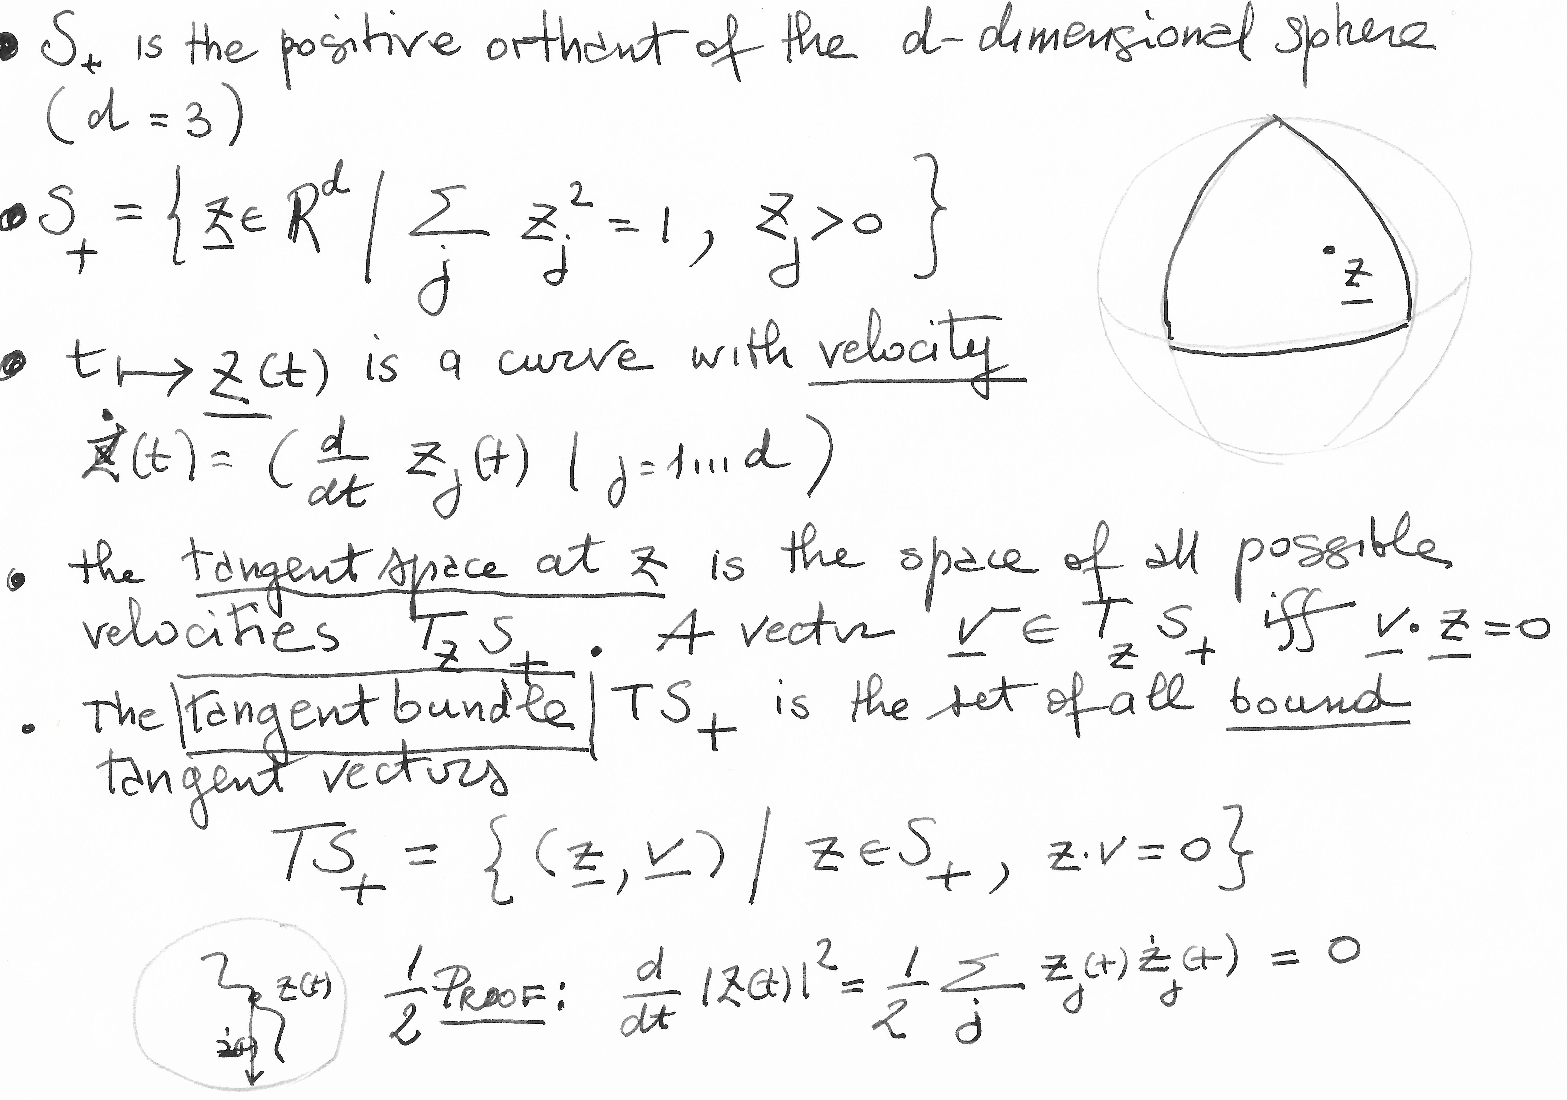
\includegraphics[width=\textwidth]{exercise/positive-orthant-cropped.pdf}

\end{frame}

\begin{frame}[plain]\frametitle{Tangent bundle as an atlas}

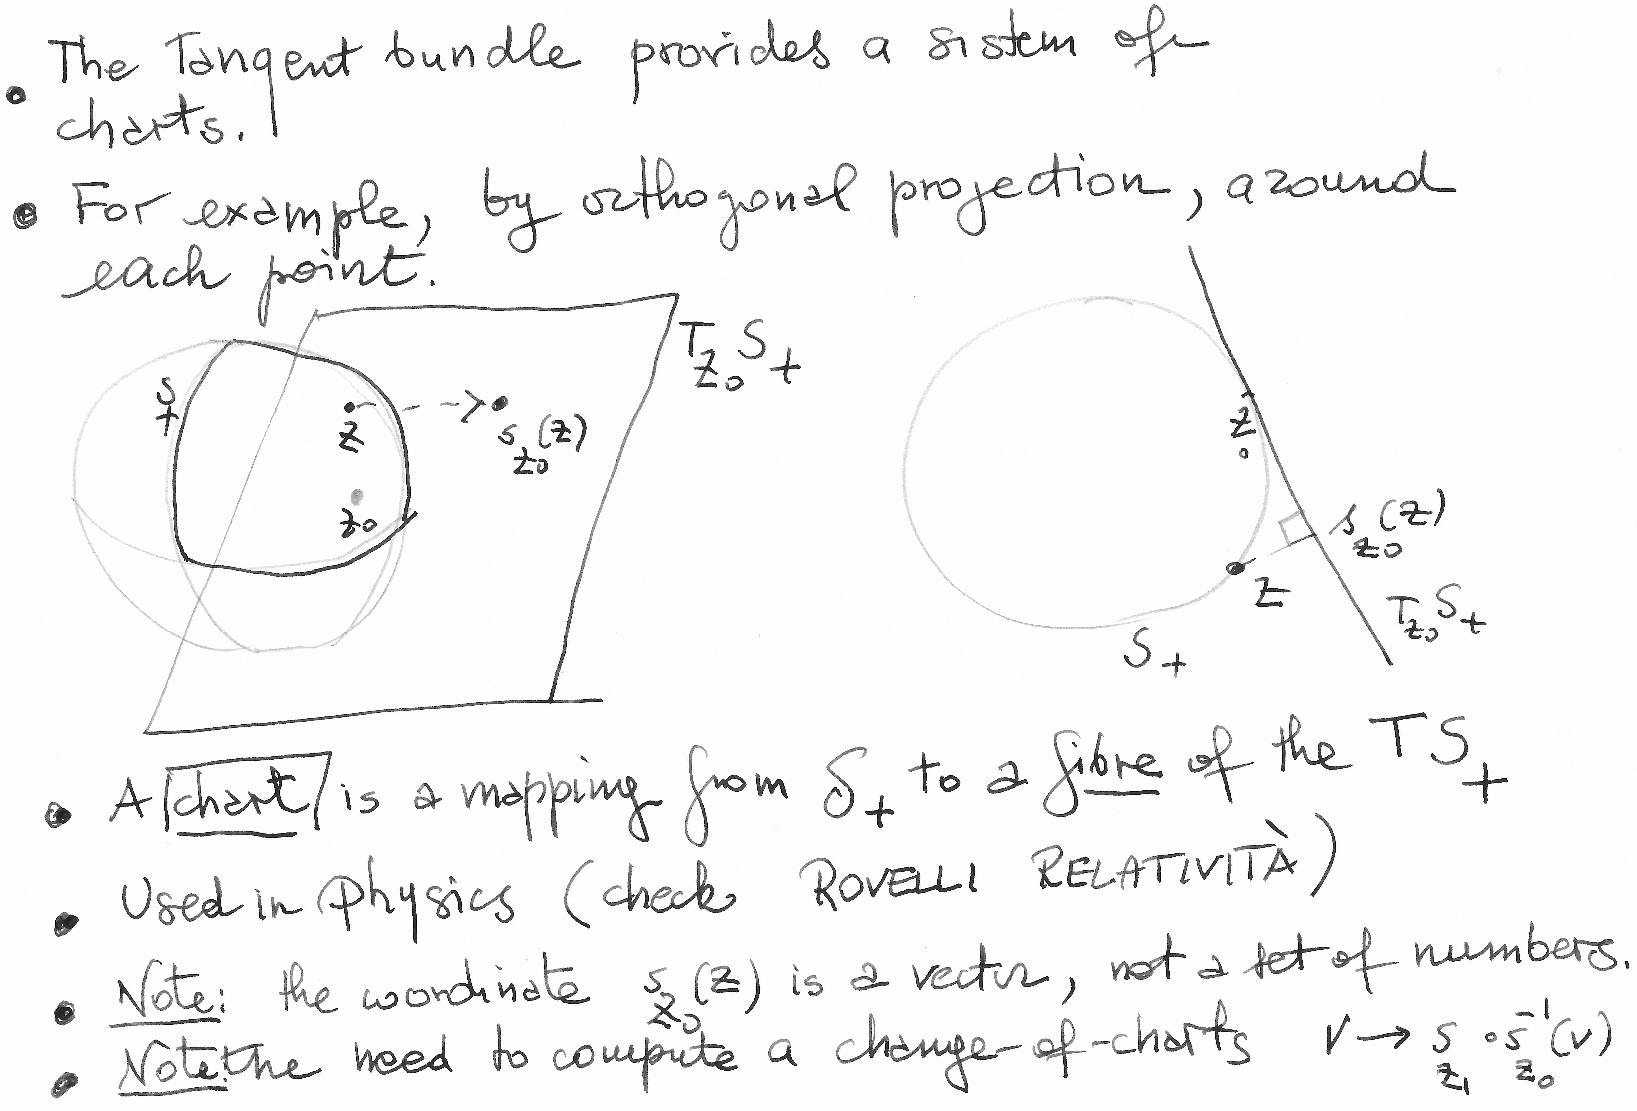
\includegraphics[width=\textwidth]{exercise/atlas-cropped.pdf}

\end{frame}

\begin{frame}[plain]\frametitle{Square-root-likelihood}

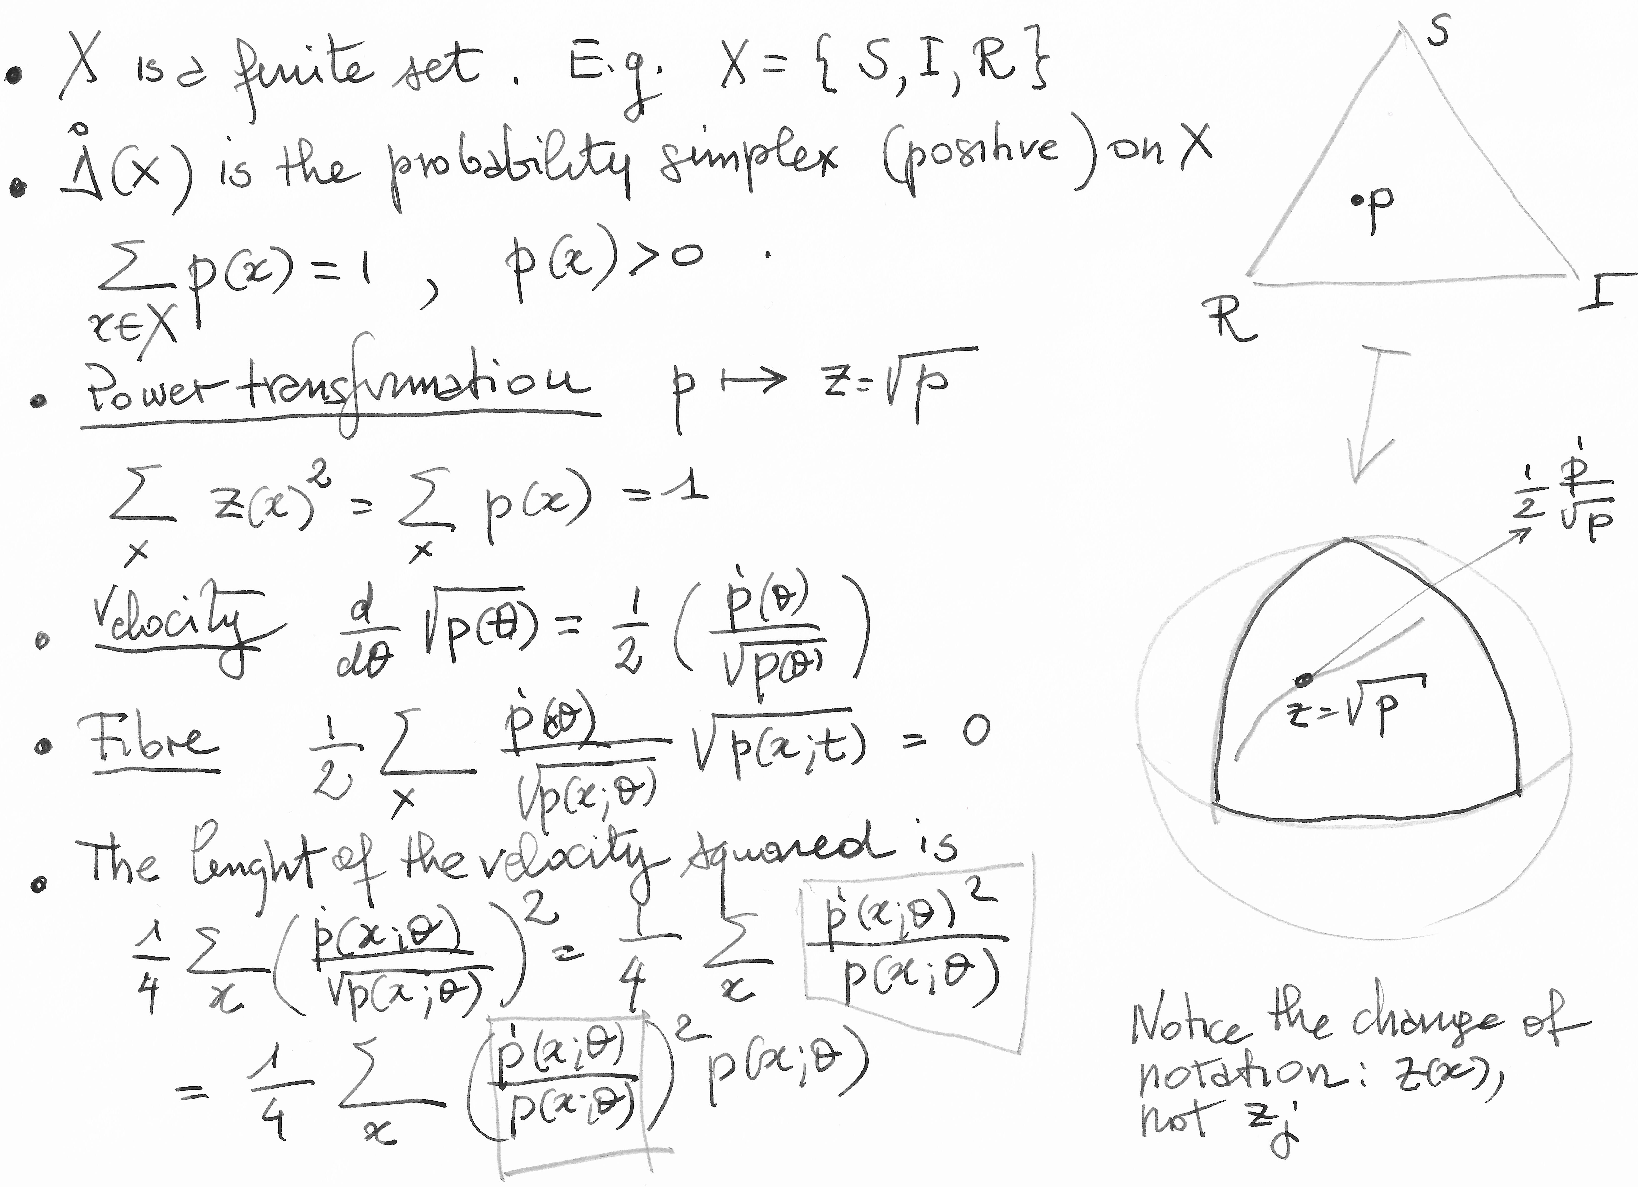
\includegraphics[width=\textwidth]{exercise/square-root-cropped.pdf}

\end{frame}

\begin{frame}[plain]\frametitle{Fisher-Cramer-Rao trick}

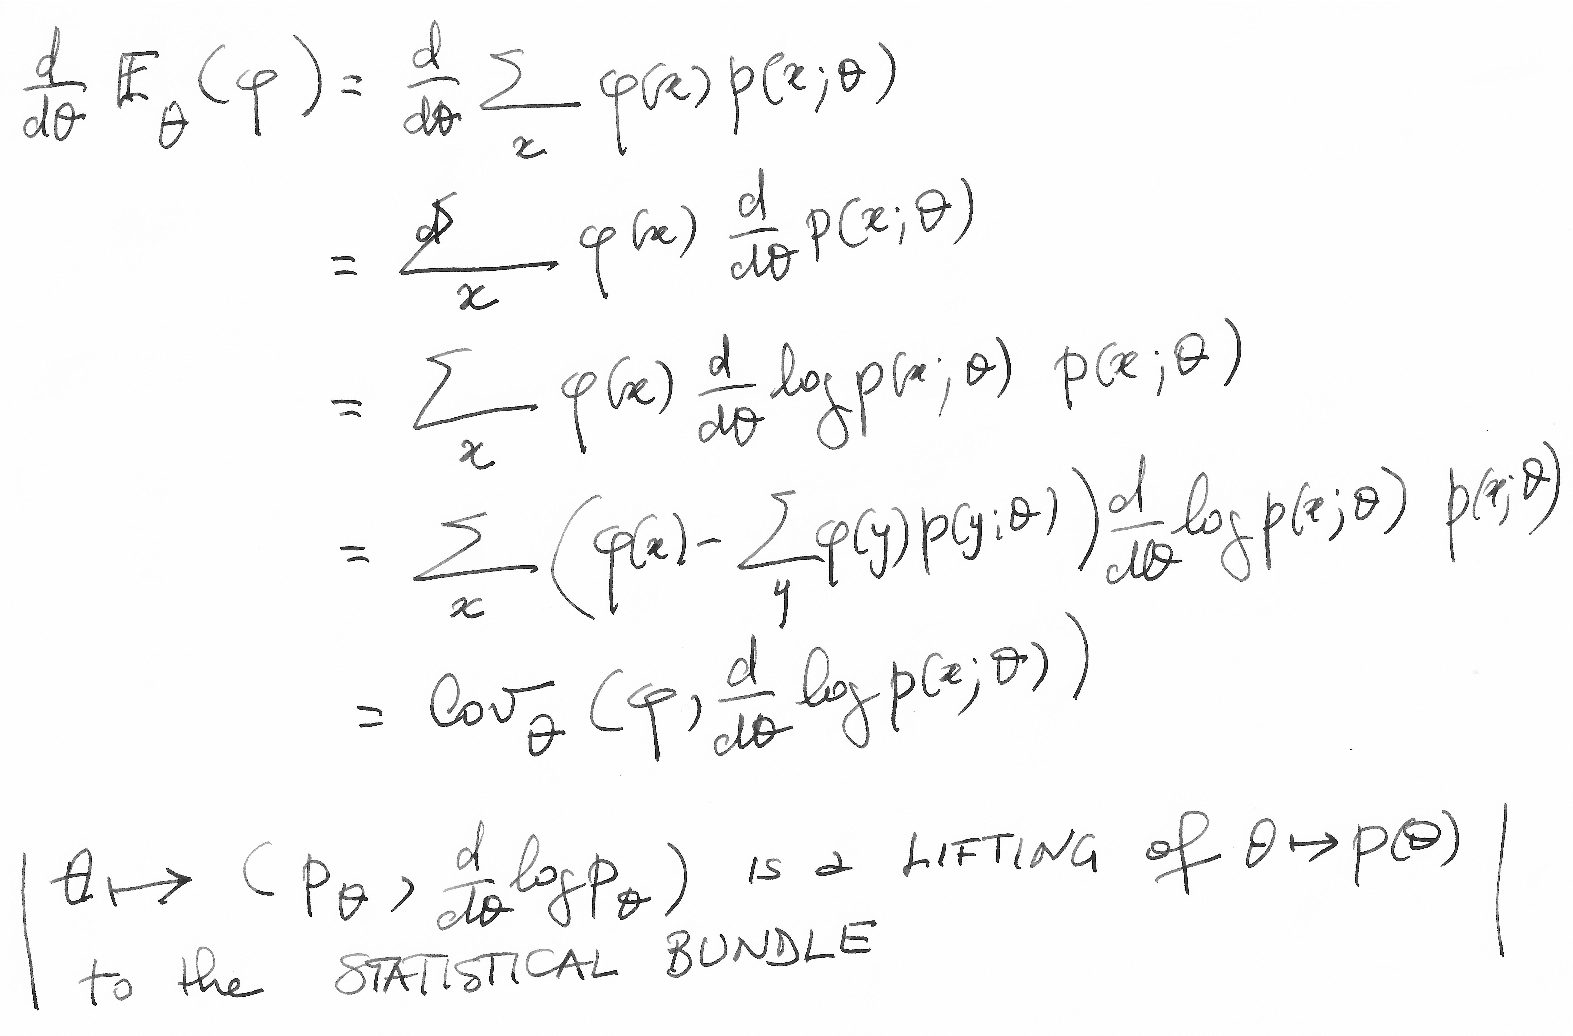
\includegraphics[width=\textwidth]{exercise/fisher-cramer-rao.pdf}

\end{frame}

\begin{frame}[plain]

  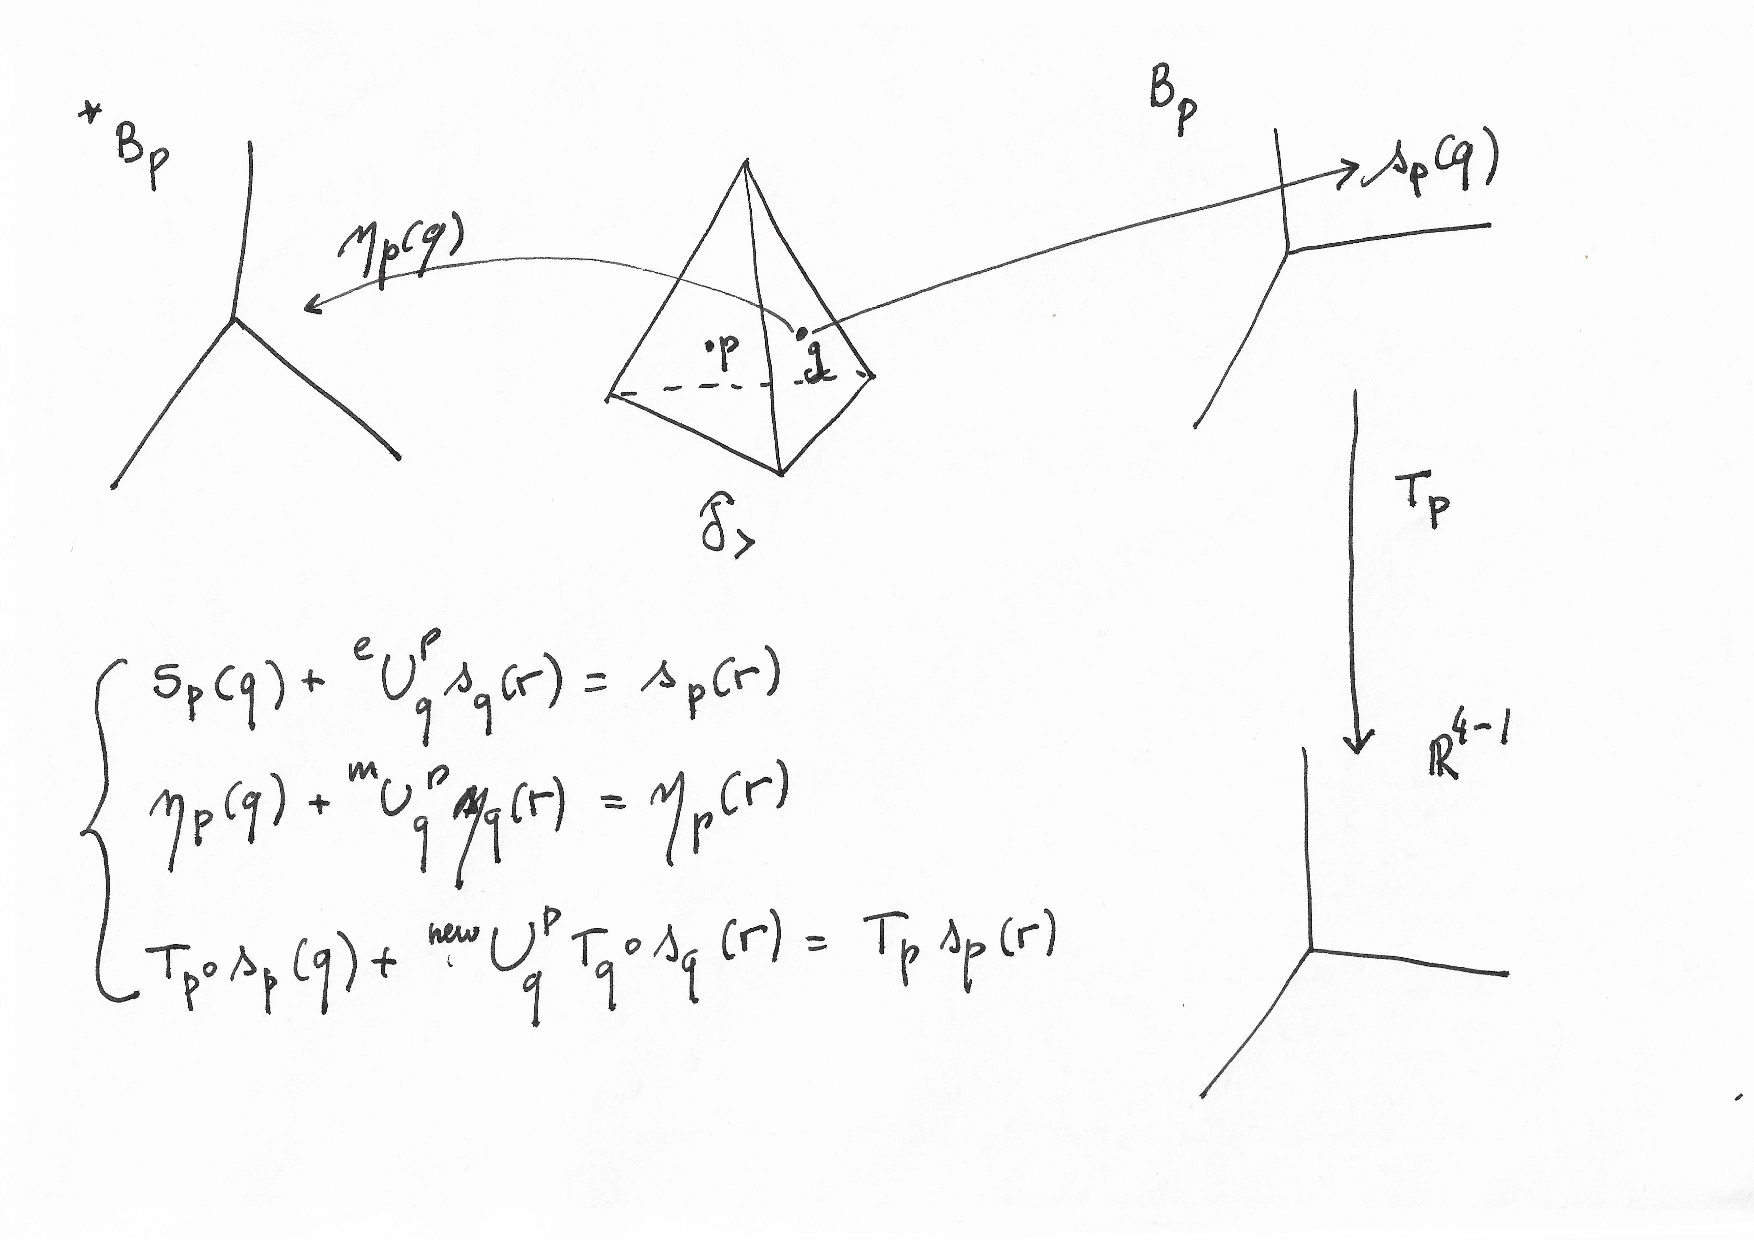
\includegraphics[height=.8\textheight]{exercise/scheme.pdf}
  
\end{frame}

\begin{frame}[plain,allowframebreaks]\small\frametitle{Exponential affine bundle}

\begin{block}{}We define the \emph{exponential displacement} on $\opensimplexon X$ by
    \begin{equation*}
      \opensimplexon X \times \opensimplexon X \ni (p,q) \mapsto s_p(q) = \boxed{\log \frac q  p - \expectat p {\log \frac q p}} \in \Bspaceat p \ ,
    \end{equation*}
    and the \emph{exponential transport} between fibers $S_p \opensimplexon X = \eBspace p$, $p \in \opensimplexon X$, by
    \begin{equation*}
      \etransport p q \colon \Bspaceat p \ni \boxed{ v \mapsto v - \expectat q v } \in \Bspaceat q \ .
    \end{equation*}
    \end{block}
    
  \begin{itemize}  \item The (generalized) parallelogram law holds:
    \begin{multline*}
      \left(\log \frac q p - \expectat p {\log \frac q p}\right) + \etransport q p \left(\log \frac r q - \expectat q {\log \frac r q}\right) = \\   \left(\log \frac q p - \expectat p {\log \frac q p}\right) + \left(\log \frac r q - \expectat p {\log \frac r q}\right) = \\ \log \frac r p - \expectat p {\log \frac r p} \ . 
    \end{multline*}
\item The inverse chart (the patch) $s_p^{-1}$ is defined on all of $\Bspaceat p$ by
  \begin{equation*}
    s^{-1}_p(v) = \boxed{\expof{v - K_p(v)} \cdot p} = e_p(v) \ , \quad K_p(v) = \log \expectat p {\euler^v} \ .
  \end{equation*}
\item The \emph{cumulant functional}
\begin{equation*}
   K_p \colon  \eBspace p \ni v \mapsto K_p(v) = \log \expectat p {\euler^v}
\end{equation*}has several important properties. It is an expression of the \emph{Kullback-Leibler divergence} as a function of the second variable:
\begin{equation*}
    \KL p q = \expectat p {\log \frac p q} = \expectat p {\log \frac p {\expof{v - K_p(v)} \cdot p}} = K_p(v) \ ,
\end{equation*}
that is,
    \emph{\begin{equation*}
      \boxed{K_p(v) = \KL p {e_p(v)} \qquad K_p(s_p(q)) = \KL p q} \ .
    \end{equation*}}
\end{itemize}

\begin{block}{Derivatives of the cumulant function}
  \begin{enumerate}
     \item \emph{$d K_p(v)[h] = \expectat {e_p(v)} {h} = \scalarat {p} {\frac{e_p(v)}{p}-1}{h}$}

    \item \emph{$d^2 K_p(v) [h,k] = \covat {e_p(v)} h k = \scalarat {e_p(v)} {\etransport p {e_p(v)} h}{\etransport p {e_p(v)} k} = \scalarat p h {\left(\mtransport {e_p(v)} p \etransport p {e_p(v)}\right) k}$}.

    \item \emph{$d^3 K_p(v) [h_1,h_2,h_3] = \expectat {e_p(v)}{\prod_{j=1}^3 \left(\etransport p {e_p(v)} h_j\right)}$}
    \end{enumerate}
\end{block}
\end{frame}

\begin{frame}[plain,allowframebreaks]\small\frametitle{Mixture affine bundle}
\begin{block}{}
      We define the \emph{mixture displacement} on $\opensimplexon X$ by
       \begin{equation*}
      \opensimplexon X \times \opensimplexon X \ni (p,q) \mapsto \eta_p(q) = \frac q p - 1 \in \Bspaceat p \ ,
    \end{equation*}
    and the \emph{mixture transport} by
    \begin{equation*}
      \mtransport p q \colon \Bspaceat p \ni v \mapsto \frac p q \, v \in \Bspaceat q \ .
    \end{equation*}
\end{block}

\begin{itemize}  
\item The (generalized) parallelogram law is
  \begin{equation*}
 \left(\frac q p -1\right) + \frac q p \left(\frac r q -1\right) = \left(\frac r p -1\right) \ .
\end{equation*}
\item The inverse chart is defined for all $v > 1$, $w \in \Bspaceat p$ by
  \begin{equation*}
    \eta^{-1}_p(v) =  (1+v) \cdot p \ .
  \end{equation*}
\end{itemize} 

\begin{block}{} We extend the mixture charts to the affine statistical bundle by
    \begin{equation*}
\eta_p \colon S\opensimplexon X \ni (q,v) \mapsto \left(\eta_p(q), \mtransport q p v \right) \in B_p \times B_p \ .        
    \end{equation*}
    The charts define an affine space with fibres $B_p^2$, $p \in \opensimplexon X$.
\end{block}

\end{frame}

\begin{frame}

    \huge PART 2: \\
    PRODUCT SAMPLE SPACE
    
\end{frame}


\begin{frame}[plain,allowframebreaks]\small\frametitle{Aside on Linear Programming LP}

\begin{itemize}  \item See \S IV.8 in \bibentry{barvinok:2002}
\end{itemize}

  \begin{itemize}
  \item The \emph{primal problem in canonical form} is
    \begin{align*}
      \text{Find} \quad c =& \inf \sum_x c(x) r(x) \\
      \text{Subject to} \quad &\sum_x A(y,x) r(x) = \beta(y) \quad y \in Y \\
      &r(x) \geq 0
    \end{align*}
  \item $r$ is the \emph{primal plan}
  \item a plan is \emph{feasible} if the constraints hold
  \end{itemize}

  \begin{itemize}
  \item The \emph{dual problem in standard form} is
    \begin{align*}
      \text{Find} \quad \beta =& \sup \sum_y \beta(y) \lambda(y) \\
      \text{Subject to} \quad &\sum_y A(y,x) \lambda(y) \leq c(x) 
    \end{align*}
  \item $\lambda$ is the \emph{dual plan}
  \end{itemize}

  \begin{block}{Strong duality theorem}
  If a feasible primal plan exists, then $c = \beta$. If moreover, $c > -\infty$, then primal optimal and dual optimal plans exist.  
  \end{block}
\end{frame}

\begin{frame}[plain,allowframebreaks]\small\frametitle{Fixed margins}
\begin{itemize}
    \item Assume a product sample space $X = \Omega_1 \times \Omega_2$ and consider the probability simplex $\simplexon{\Omega_1 \times \Omega_2}$. The two marginalisation mappings are
    \begin{align*}
 X_1& \colon \simplexon{\Omega_1 \times \Omega_2} \ni q(\cdot,\cdot) \mapsto \sum_{x_2} q(\cdot,x_2) \in  \simplexon{X_1}  \\
 X_2& \colon \simplexon{\Omega_1 \times \Omega_2} \ni q(\cdot,\cdot) \mapsto \sum_{x_1} q(x_1,\cdot) \in  \simplexon{X_2} 
    \end{align*}
    \item For each given $q_1 \in \simplexon{X_1}$ and $q_2 \in \simplexon{X_2}$ define 
    \begin{equation*}
        \Pi(q_1,q_2) = \setof{q \in \simplexon{\Omega_1 \times \Omega_2}} {X_1 q = q_1, X_2 q = q_2} \ .
    \end{equation*}
    \item The set of \emph{transport plans}  $\Pi(q_1,q_2)$ is \begin{itemize} \item non-empty, \item convex, \item compact.
    \end{itemize}

    \item The marginalization conditions
    \begin{gather*}
        \sum_{x_2 \in X_2} q(y_1,x_2) = q_1(y_1) \quad y_1 \in X_1 \\
            \sum_{x_1 \in X_1} q(x_1,y_2) = q_2(y_2) \quad y_2 \in X_2
    \end{gather*}
    can be written as
    \begin{gather*}
        \sum_{(x_1,x_2) \in X_1\times X_2} (y_1 = x_1) q(x_1,x_2) = q_1(y_1) \\
             \sum_{(x_1,x_2) \in X_1\times X_2} (y_2 = x_2) q(x_1,x_2) = q_2(y_2)
    \end{gather*}
    thus identifying an operator $A \colon (X_1 \cup X_2) \times (\Omega_1 \times \Omega_2)$ with
    \begin{equation*}
     \sum_{(x_1,x_2) \in \Omega_1 \times \Omega_2} A(y;x_1,x_2) q(x_1,x_2) = (q_1 \cup q_2)(y)    
    \end{equation*}
\end{itemize}    
\end{frame}

\begin{frame}[plain,allowframebreaks]\small\frametitle{Kantorovich optimal transport}
\begin{itemize}
    \item Given the \emph{cost} $c \colon \Omega_1 \times \Omega_2 \to \reals$, Kantorovich looks for the transport plan with minimal expected cost
    \begin{equation*}
        \inf \setof{\sum_{x_1,x_2} c(x_1,x_2) q(x_1,x_2)}{q \in \Pi(q_1,q_2)}
    \end{equation*}
    \item It is a primal problem in canonical form:
       \begin{align*}
      \text{Find} \quad c =& \inf \sum_{x_1,x_2} c(x_1,x_2) q(x_1,x_2) \\
      \text{Subject to} \quad &\sum_x A(y;x_1,x_2) q(x_1,x_2) = (q_1 \cup q_2)(y) \\
      &q(x_1,x_2) \geq 0 \ .
    \end{align*}
\end{itemize}

\begin{itemize}
    \item The dual problem in standard form is
    \begin{align*}
      \text{Find} \quad \beta =& \sup \sum_y (q_1 \cup q_2) (y) \lambda(y) \\
      \text{Subject to} \quad &\sum_y A(y;x_1,x_2) \lambda(y) \leq c(x_1,x_2) 
    \end{align*}
\item    that is, given the form of $A$,
\begin{align*}
      \text{Find} \quad \beta =& \sup \left(\sum_{y_1\in X_1}q_1(y_1) \lambda_1(y_1) + \sum_{y_2 \in X_2} q_2(y_2) \lambda_2(y_2)\right) \\
      \text{Subject to} \quad &\lambda_1(x_1) + \lambda_2(x_2) \leq c(x_1,x_2) \ .
    \end{align*}
\end{itemize}

\begin{itemize}
    \item There exists a feasible transport plan, and the set of plans is compact. It follows that the full strong duality theorem holds.
    \item Let $\bar q$, $\bar \lambda$ be the optimal plan and dual plan. The equality of values gives
    \begin{multline*}
    \sum_{x_1,x_2} c(x_1,x_2)\bar q(x_1,x_2) = \\ \sum_{x_1\in X_1}q_1(x_1) \bar \lambda_1(x_1) + \sum_{x_2 \in X_2} q_2(x_2) \bar \lambda_2(x_2) = \\
    \sum_{x_1,x_2} \left(\bar \lambda_1(x_1) + \bar \lambda_2(x_2)\right) \bar q(x_1,x_2) 
    \end{multline*}
    \item Now, the inequality $c \geq \lambda_1 \oplus \lambda _2$ implies
    \begin{equation*}
        c(x_1,x_2)=\bar \lambda_1(x_1) + \bar \lambda_2(x_2) \quad \text{provided $\bar q(x_1,x_2) \neq 0$}
    \end{equation*}
\end{itemize}
    
\end{frame}

\begin{frame}[plain]\small\frametitle{Transport plans in $\maxexpat {\Omega_1 \times \Omega_2}$}
 \begin{itemize}
 
     \item Define for all $q_1 \in \maxexpat{\Omega_1}$ and $q_2 \in \maxexpat{\Omega_2}$
     \begin{equation*}
         \overset{\circ}{\Pi}(q_1,q_2) = \setof{q \in \maxexpat{\Omega_1 \times \Omega_2}}{X_1 q = q_1,X_2 q= q_2}
     \end{equation*}
 
 \item  $\overset{\circ}{\Pi}$ is the set of positive \emph{couplings} or positive \emph{transport plans} of $q_1$ and $q_2$. 
 \item \emph{$\overset{\circ}{\Pi}$ is the base set of a sub-manifold of the affine statistical manifold on $\maxexpat {\Omega_1 \times \Omega_2}$}.

\item A \emph{sub-manifold} of the affine manifold $(M,s_p,\eBspace p,\transport p q \colon p,q \in M)$ is a subset $N \subset M$ such that for each $q \in N$ there exists a smooth splitting of the fibre $\eBspace q = S_q N \oplus R_q N$ and the vector space $S_q N$ is the set of all velocities of curves in $N$ through $q$. 

\item Basic examples of sub-manifolds of affine statistical manifolds are mixture models and exponential families, to be discussed elsewhere. Here we discuss the set of couplings or transport plans.
 \end{itemize}
\end{frame}

 \begin{frame}[plain,allowframebreaks]\small\frametitle{Example} 
 
 %\begin{figure}
  \begin{tabular}{ccc}
    \begin{tikzpicture}[scale=1.7,baseline = (current bounding box.center)]
\node (n00) at (1,-.5) {$\delta_{11}$};
\node (n10) at (0,0) {$\delta_{21}$};
\node (n01) at (2,0) {$\delta_{12}$};
\node (n11) at (1,1.5) {$\delta_{22}$};
\node (K1) at (5/6,-1/12) {$\gamma_1$};
\node (K2) at (5/6,1/4) {$\gamma_2$};
\draw[thick,dotted] (n01) -- (n10);
\foreach \from/\to in {n00/n10,n00/n01,n11/n10,n11/n01,n00/n11}
\draw[thick] (\from) -- (\to);
\draw [thick,red] (K1) -- (K2); % was: gray, dashed
\end{tikzpicture} & $\xrightarrow[(X_1,X_2)_{\#}]{}$ &
    \begin{tikzpicture}[scale=3,baseline = (current bounding box.center)]
\node (n00) at (0,0) {$\delta_{11}$};
\node (n10) at (1,0) {$\delta_{12}$};
\node (n01) at (0,1) {$\delta_{21}$};
\node (n11) at (1,1) {$\delta_{22}$};
\foreach \from/\to in {n00/n01,n01/n11,n11/n10,n10/n00}
\draw[thick] (\from) -- (\to);
\filldraw [red] (1/2,2/3) circle (1pt); % was: gray
\end{tikzpicture}
  \end{tabular}
  %\caption{
  %\label{fig:2x2}}
  %\end{figure}

Cf Pistone-Rapallo-Rogantin:2021
\begin{itemize}
\item The sample space is: 
\begin{equation*}
  \Omega_1=\Omega_2 = \set{1,2} \quad \Omega_1 \times \Omega_2 = \set{11,12,21,22} 
\end{equation*}
\item The margins are:
\begin{equation*}
   {\color{red}\bullet} = \left((1/2, 1/2), (2/3, 1/3)\right) = \left((q_1(1),q_1(2)),(q_2(1),q_2(2))\right) 
\end{equation*}

\item Cf. Exercise 2x2 coupling.

\item The vertexes of the transport polytope are:
\begin{equation*}
\gamma_1 = \begin{bmatrix} 1/6 & 1/3 \\ 1/2 & 0 \end{bmatrix} \quad 
\gamma_2 = \begin{bmatrix} 1/2 & 0 \\ 1/6 & 1/3 \end{bmatrix}\end{equation*}
\item The transport polytope is 
\begin{align*}
 \openplan{q_1}{q_2} &= \setof{(1-t)\begin{bmatrix} 1/6 & 1/3 \\ 1/2 & 0 \end{bmatrix} + t \begin{bmatrix} 1/2 & 0 \\ 1/6 & 1/3 \end{bmatrix}}{0 < t < 1} \\
 &= \setof{\begin{bmatrix} 1/6 & 1/3 \\ 1/2 & 0 \end{bmatrix} + t \begin{bmatrix} 1/3 & -1/3 \\ -1/3 & 1/3 \end{bmatrix}}{0 < t < 1}
\end{align*}
\item A curve in the transport polytope is 
\begin{equation*}
   \gamma \colon t \mapsto \begin{bmatrix} 1/6 & 1/3 \\ 1/2 & 0 \end{bmatrix} + a(t) \begin{bmatrix} 1/3 & -1/3 \\ -1/3 & 1/3 \end{bmatrix}
\end{equation*}

\end{itemize}
\end{frame}

  \begin{frame}[plain]\small\frametitle{$\openplan {q_1} {q_2}$ as a sub-manifold of $\maxexpat{\Omega_1 \times \Omega_2}$}
      
  \begin{itemize}

\item Finite dimensional exponential families and finite-dimensional mixture models are notable examples of sub-manifolds of the affine manifold structure because they are flat in one of the two dual geometries. 

\item Notice that the orthogonal projection on the space of velocities provides the required splitting.

\item Precisely, the space $S_q N$ of velocities is the affine expression of the tangent space to $N$. 

\item The set of couplings $\Pi(q_1,q_2)$ is an affine subset of the probability simplex. Hence it is a polytope, a convex set generated by a finite number of vertices. 

\item Hence, \emph{$\openplan {q_1}{q_2}$ is an open mixture model}. 

\end{itemize}
\end{frame}

\begin{frame}[plain,allowframebreaks]\small\frametitle{Velocities of curves in $\overset{\circ}\Pi(q_1,q_2)$}

\begin{itemize}
    \item $t \mapsto q(t)$ is a smooth curve of $\maxexpat {\Omega_1 \times \Omega_2}$ with values in the set of strictly positive transport plans. We can say
    \begin{equation*}
      t \mapsto q(t) \in \overset{\circ}{\Pi}(q_1,q_2)
    \end{equation*}
    \item Recall Fisher's score properties,
    \begin{gather*}
        \velocity q(t) = \derivby t \log q(t) = \frac {\dot q(t)}{q(t)} \\
        \derivby t \expectat {q(t)} f = \scalarat {q(t)} {f - \expectat {q(t)} f}{\velocity q(t)} \ . 
    \end{gather*}
    \item For each random variable depending on the first variable only, $f_1\circ X_1$ it holds
\begin{multline*} 0 = \derivby t \expectat {q_1} {f_1} =  \derivby t \expectat {q(t)} {f_1\circ X_1} = \\ \scalarat {q(t)}  {f_1 \circ X_1 - \expectat {q(t)} {f_1\circ X_1}} {\velocity q(t)} = \expectat {q(t)} {f_1\circ X_1 \velocity q(t)} \ , \end{multline*}  Similarly on the other projection.
\item It follows that
\begin{equation*}
\boxed{\condexpectat {q(t)} {\velocity q(t)} {X_1} = 0 \quad \text{and} \quad \condexpectat {q(t)} {\velocity q(t)} {X_2} = 0}
\end{equation*}
that is, \emph{if $t \mapsto q(t) \in \openplan{q_1}{q_2}$, then $\velocity q(t)$ is an interaction at $q(t)$, $\velocity q(t) \in H_2(q(t))$}.
\item Conversely, let $q \in \openplan{q_1}{q_2}$ and $c_{12} \in H(q)$. The curve $t \mapsto (1+tc) \cdot q$ is defined in a neighborhood of 0. The margins are correct,
\begin{equation*}
    \expectat {(1+tc_{12}) \cdot q}{g\circ X_i} = \expectat q {(1+tc_{12})g\circ X_i} = \expectat {q_1} g \ ,
\end{equation*}
and the velocity at 0 is $c_{12}$,
\begin{equation*}
   \left. \derivby t \logof{(1+tc_{12}) \cdot q}
\right|_{t=0} = \left. \frac {c_{12} q}{(1+tc_{12})q} \right|_{t=0} = c_{12} \ .
\end{equation*}
\item In conclusion, \emph{for all $q \in \overset{\circ}{\Pi}(q_1,q_2)$, the velocities fiber is the vector space of interactions},
\begin{equation*}
 \boxed{S_q \overset{\circ}\Pi(q_1,q_2) = H_2(q)}
\end{equation*}

\item The orthogonal splitting of the statistical bundle is
\begin{equation*}
    \expfiberat q {\Omega_1 \times \Omega_2} = S_q \openplan{q_1}{q_2} \oplus_q \hajekof{q}\expfiberat q {\Omega_1 \times \Omega_2},
\end{equation*}
where $q_1, q_2$ are the margins of $q$.

\item Notice that the complement fiber is $H_1(q)$,
\begin{multline*}
  \hajekof{q}\expfiberat q {\Omega_1 \times \Omega_2} = \\ \setof {f_1 \circ X_1 + f_2 \circ X_2}{\expectat {q_1}{f_1} = \expectat {q_2}{X_2} = 0} \ ,
 \end{multline*}
  which is in turn related to the \emph{exponential families of additive statistics} 
  \begin{equation*}
      \expof{f_1 \circ X_1 + f_2 \circ X_2 - K_q(f_1 \circ X_1 + f_2 \circ X_2)} \cdot q \ .
  \end{equation*}
\end{itemize}
\end{frame}

\begin{frame}[plain,allowframebreaks]\small\frametitle{$\openplan{q_1}{q_2}$ as an affine space}
\begin{itemize}
\item If $q , r \in \openplan {q_1} {q_2}$, given $c \in H_2(q) = S_q \openplan {q_1}{q_2}$,
\begin{equation*}
\expectat r {\left(\frac q r c\right) g_i \circ X_i} = \expectat q {c \,  g_i \circ X_i} = 0
\end{equation*}
that is, $\frac q r c \in H_2(r) = S_r \openplan {q_1}{q_2}$.
\item We have defined a co-cycle 
of parallel transports on the bundle
\begin{equation*}
    S \openplan {q_1}{q_2} = \setof {(q,c)}{ q \in \openplan {q_1}{q_2}, c \in H_2(q)} 
\end{equation*}
\item The dual transport is computed as follows. If
\begin{gather*}
  q, r \in \openplan {q_1}{q_2} \\
  c \in S_q \openplan {q_1}{q_2} = H_2(q) \\
  d \in S_r \openplan {q_1}{q_2} = H_2(r)
\end{gather*}
then
\begin{equation*}
\scalarat r {\mtransport q r c} d = \expectat q {cd} = \scalarat q c {d - \hajekof q d}
\end{equation*}
\item Let us compute the mixture geodesic. If $(q,c) \in S \openplan {q_1}{q_2}$, an m-geodesic is a curve in $t \mapsto q(t) \in \openplan {q_1}{q_2}$ such that $(q(0),\velocity q(0)) = (q,c)$ and $\velocity q(t) = \mtransport q {q(t)} c$. It follows
\begin{equation*}
    \frac {\dot q(t)}{q(t)} = \frac q {q(t)} c \quad \text{then} \quad q(t) = (1 +tc) \cdot q \ .
\end{equation*}
\emph{The m-geodesic from $q$ in the direction $c$ is $t \mapsto (1+tc)\cdot q$}. 
\item The \emph{the affine displacement is the geodesic at $t=1$}:
\begin{equation*}
 \openplan {q_1}{q_2} \times  \openplan {q_1}{q_2} \ni (q,r) \mapsto \frac r q - 1
\end{equation*}
\item The e-geodesic from $q$ in the direction $d$ is the solution of
\begin{equation*}
\velocity q(t) = (I - \hajekof{q(t)})d \ .
\end{equation*}
\item A solution of this equation seems to require a solution of the Hajek projection.
\end{itemize}

\end{frame}

\begin{frame}[plain,allowframebreaks]\small\frametitle{Gradient flow of the OT problem}

\begin{itemize}
    \item 
Let us discuss the \emph{Optimal Transport OT} problem in the framework of the affine statistical bundle.
\item $c \colon \Omega_1 \times \Omega_2 \to \reals$ be a cost function and the expected cost function as a function of the probability function is
\begin{equation*}
  C \colon \maxexpat {\Omega_1 \times \Omega_2} \ni q \mapsto \expectat q c
\end{equation*}
\item The function $q \mapsto C(q)$ restricted to the open transport model $\openplan{q_1}{q_2}$ has gradient in $S\openplan{q_1}{q_2}$ given by
\begin{equation*}
 \grad C \colon q \mapsto c_{12}(q) = c - \expectat q c - \hajekof q c 
\end{equation*}
\item In fact for all curve $t \mapsto q(t) \in \openplan {q_1}{q_2}$, $q(0) = q$,
\begin{multline*}
\derivby t C(q(t)) = \derivby t \expectat {q(t)} c = \scalarat {q(t)} {c - \expectat {q(t)} c}{\velocity q(t)} = \\
\scalarat {q(t)} {c - \expectat {q(t)} c - \hajekof {q(t)} c}{\velocity q(t)}
\end{multline*}

\item The equation of the \emph{gradient flow of $C$} is
\begin{equation*}
  \velocity q(t) = - c_{12}(q(t)) = - (c - \expectat {q(t)} c - \hajekof {q(t)} c)
\end{equation*}

\item Notice that  $c_{12}(q) = c - \expectat q c - \hajekof {q} c$ is defined for  all $q \in \Pi(q_1,q_2)$. If $\hat q$ is a zero of the extended gradient map,
\begin{equation*}
    \grad C(\hat q) = c_{12}(\hat q) = 0 \ ,
\end{equation*}
then $c$ equals the sum of two functions in one variable on the support of $\hat q$.
\item
We expect any solution $t \mapsto q(t)$ of the gradient flow equation to converge to a plan $\bar q = \lim_{t \to \infty} q(t) \in \Pi(q_1,q_2)$ such that $\expectat {\bar q} c$ is the value of the Kantorovich optimal transport problem. The form of the gradient is compatible with the classical result in OT.
\end{itemize}
\end{frame}

\begin{frame}[plain]\frametitle{Exercise: conditional expectation}

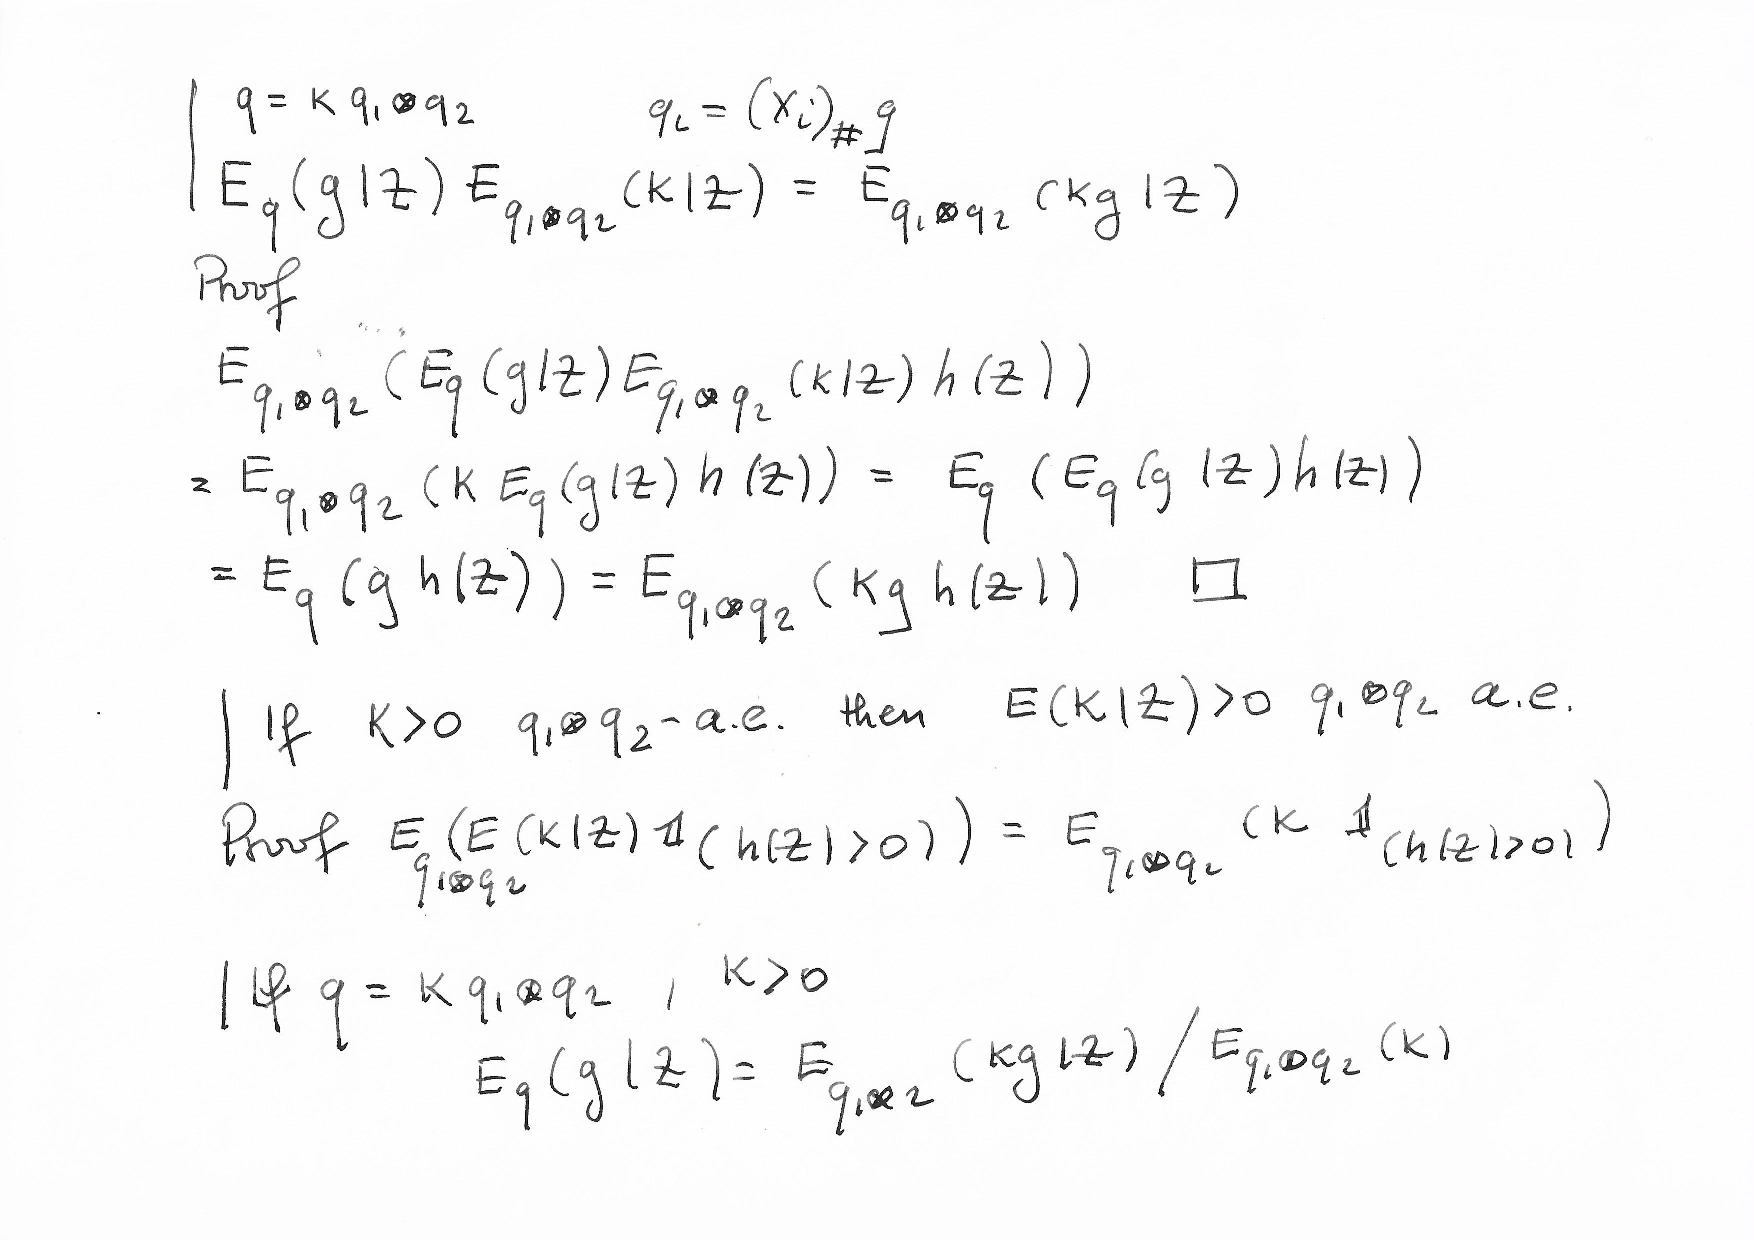
\includegraphics[width=\textwidth]{exercise/bayes-conditional-expectation.pdf}

\end{frame}

\begin{frame}[plain,allowframebreaks]\frametitle{Exercise: $2\times2$ coupling}

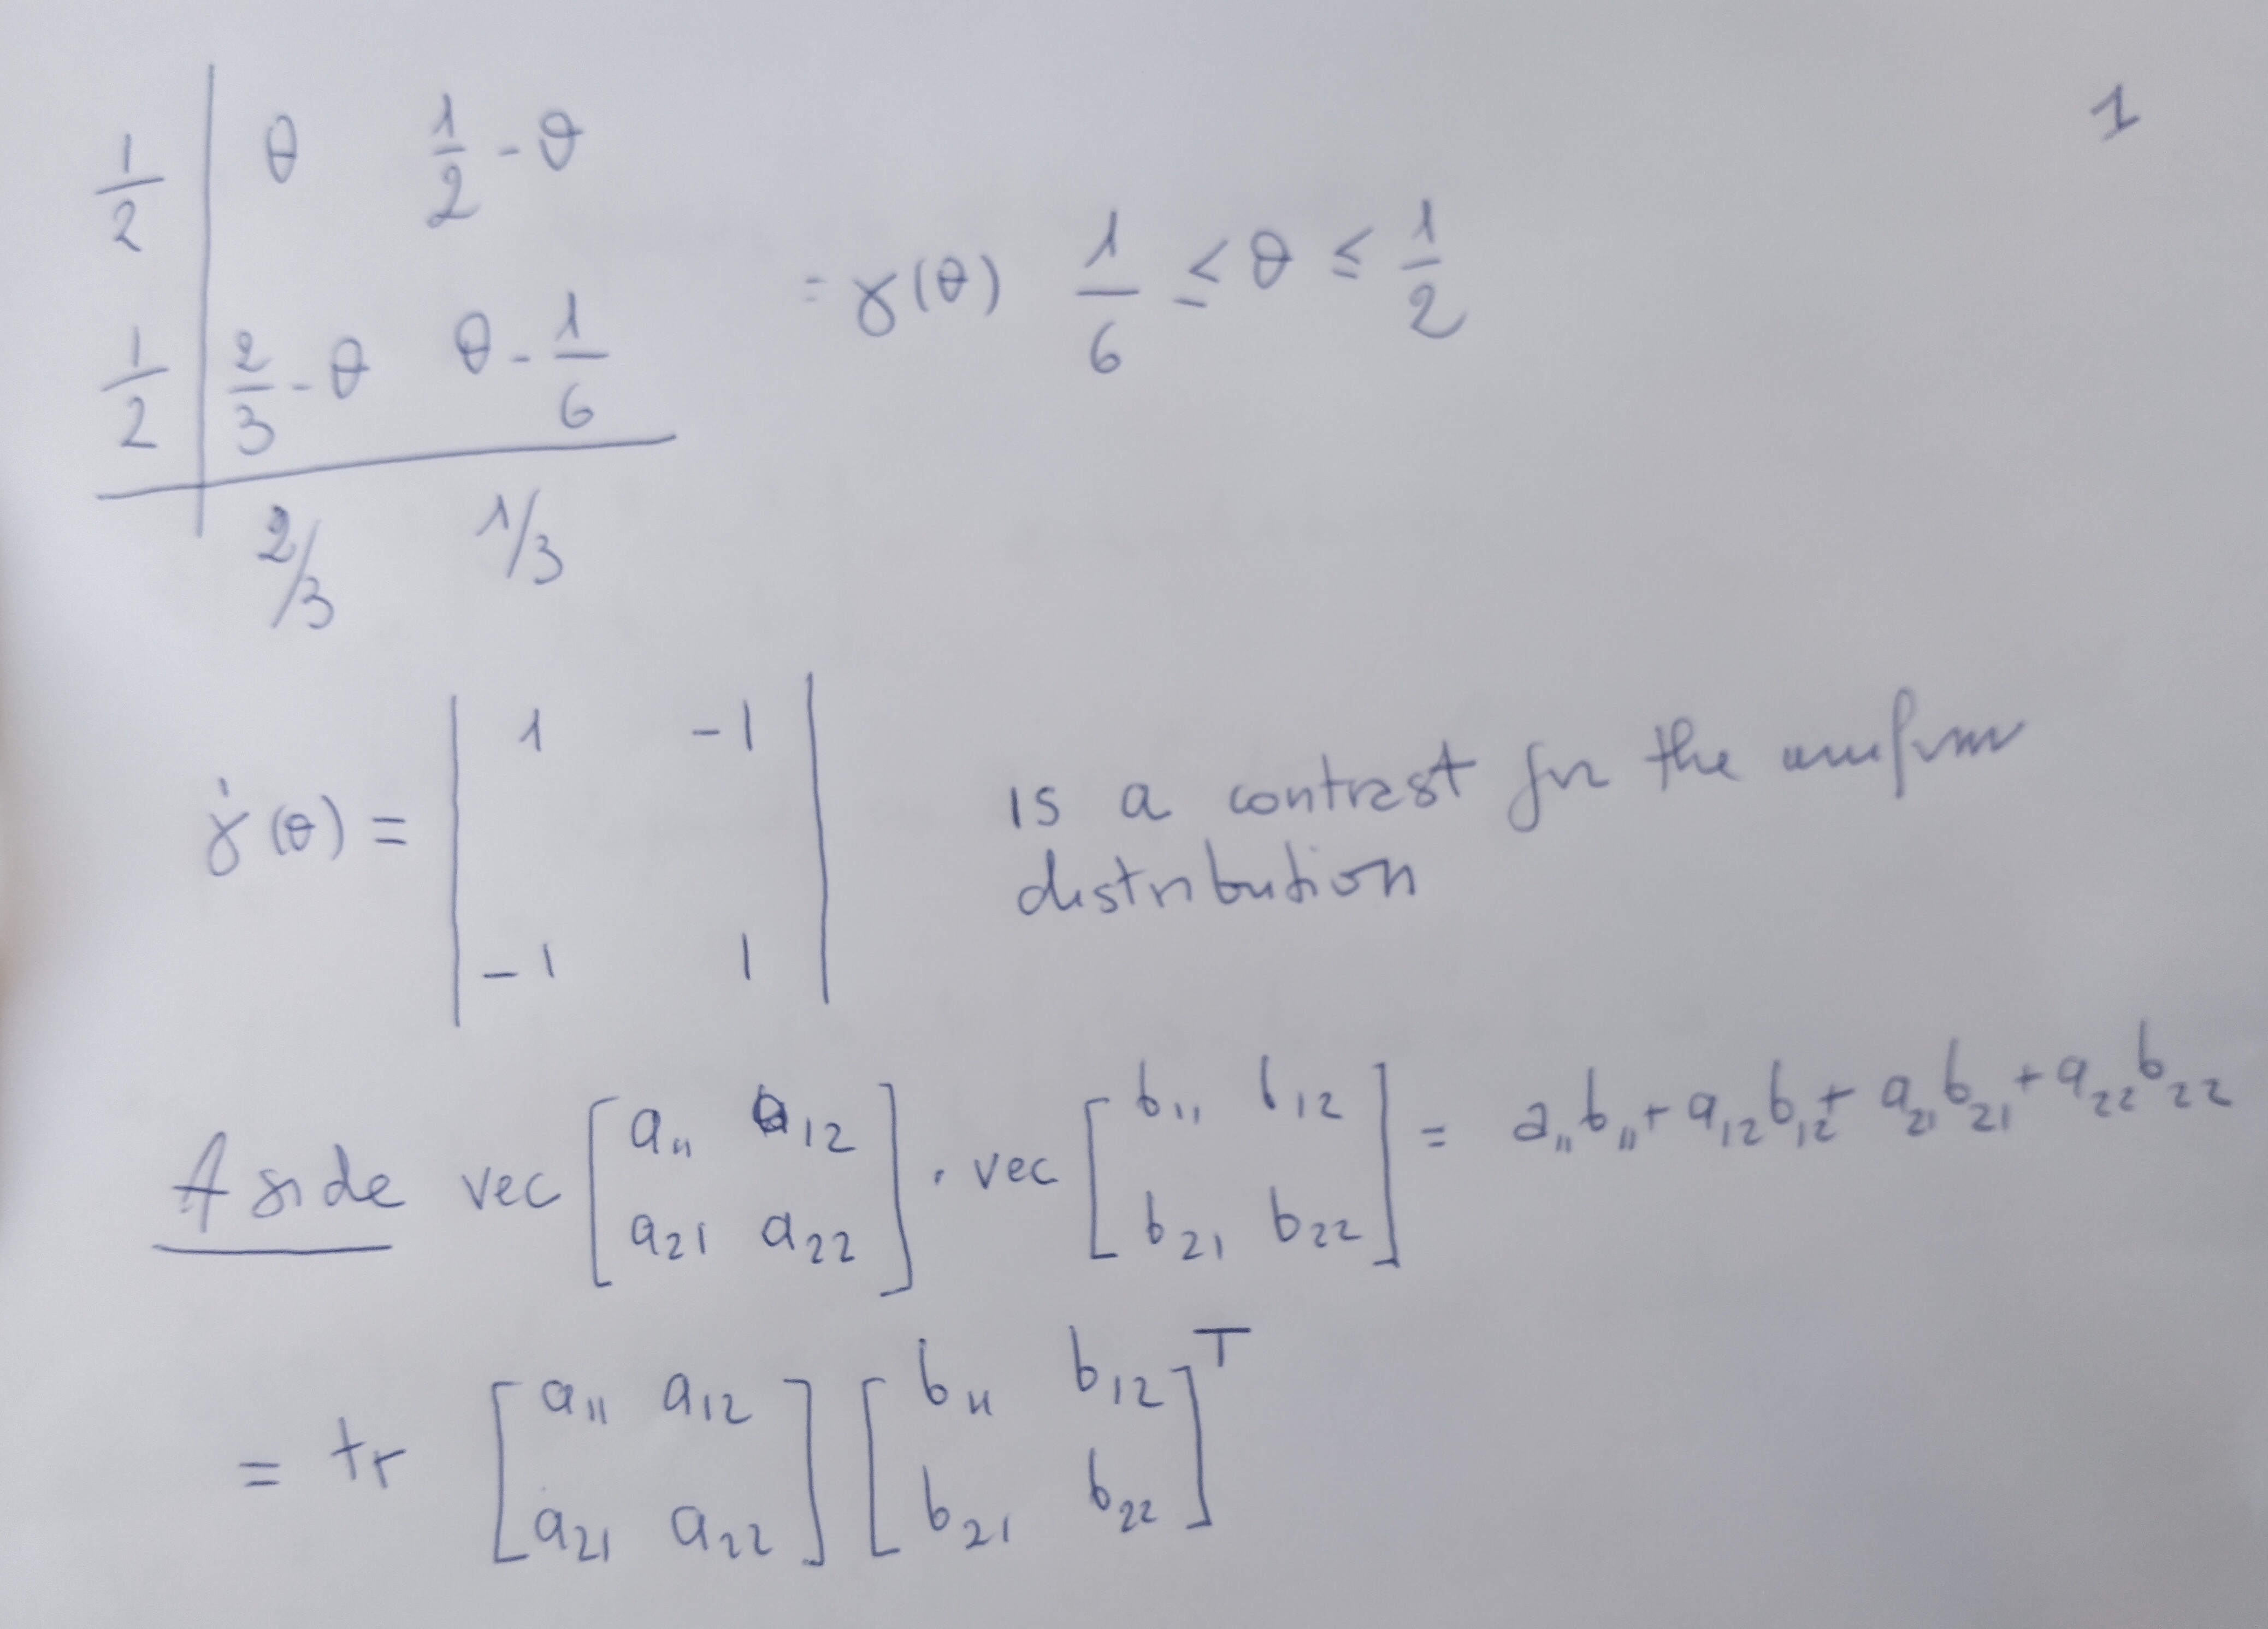
\includegraphics[width=\textwidth]{exercise/2x2-coupling-1.jpg}

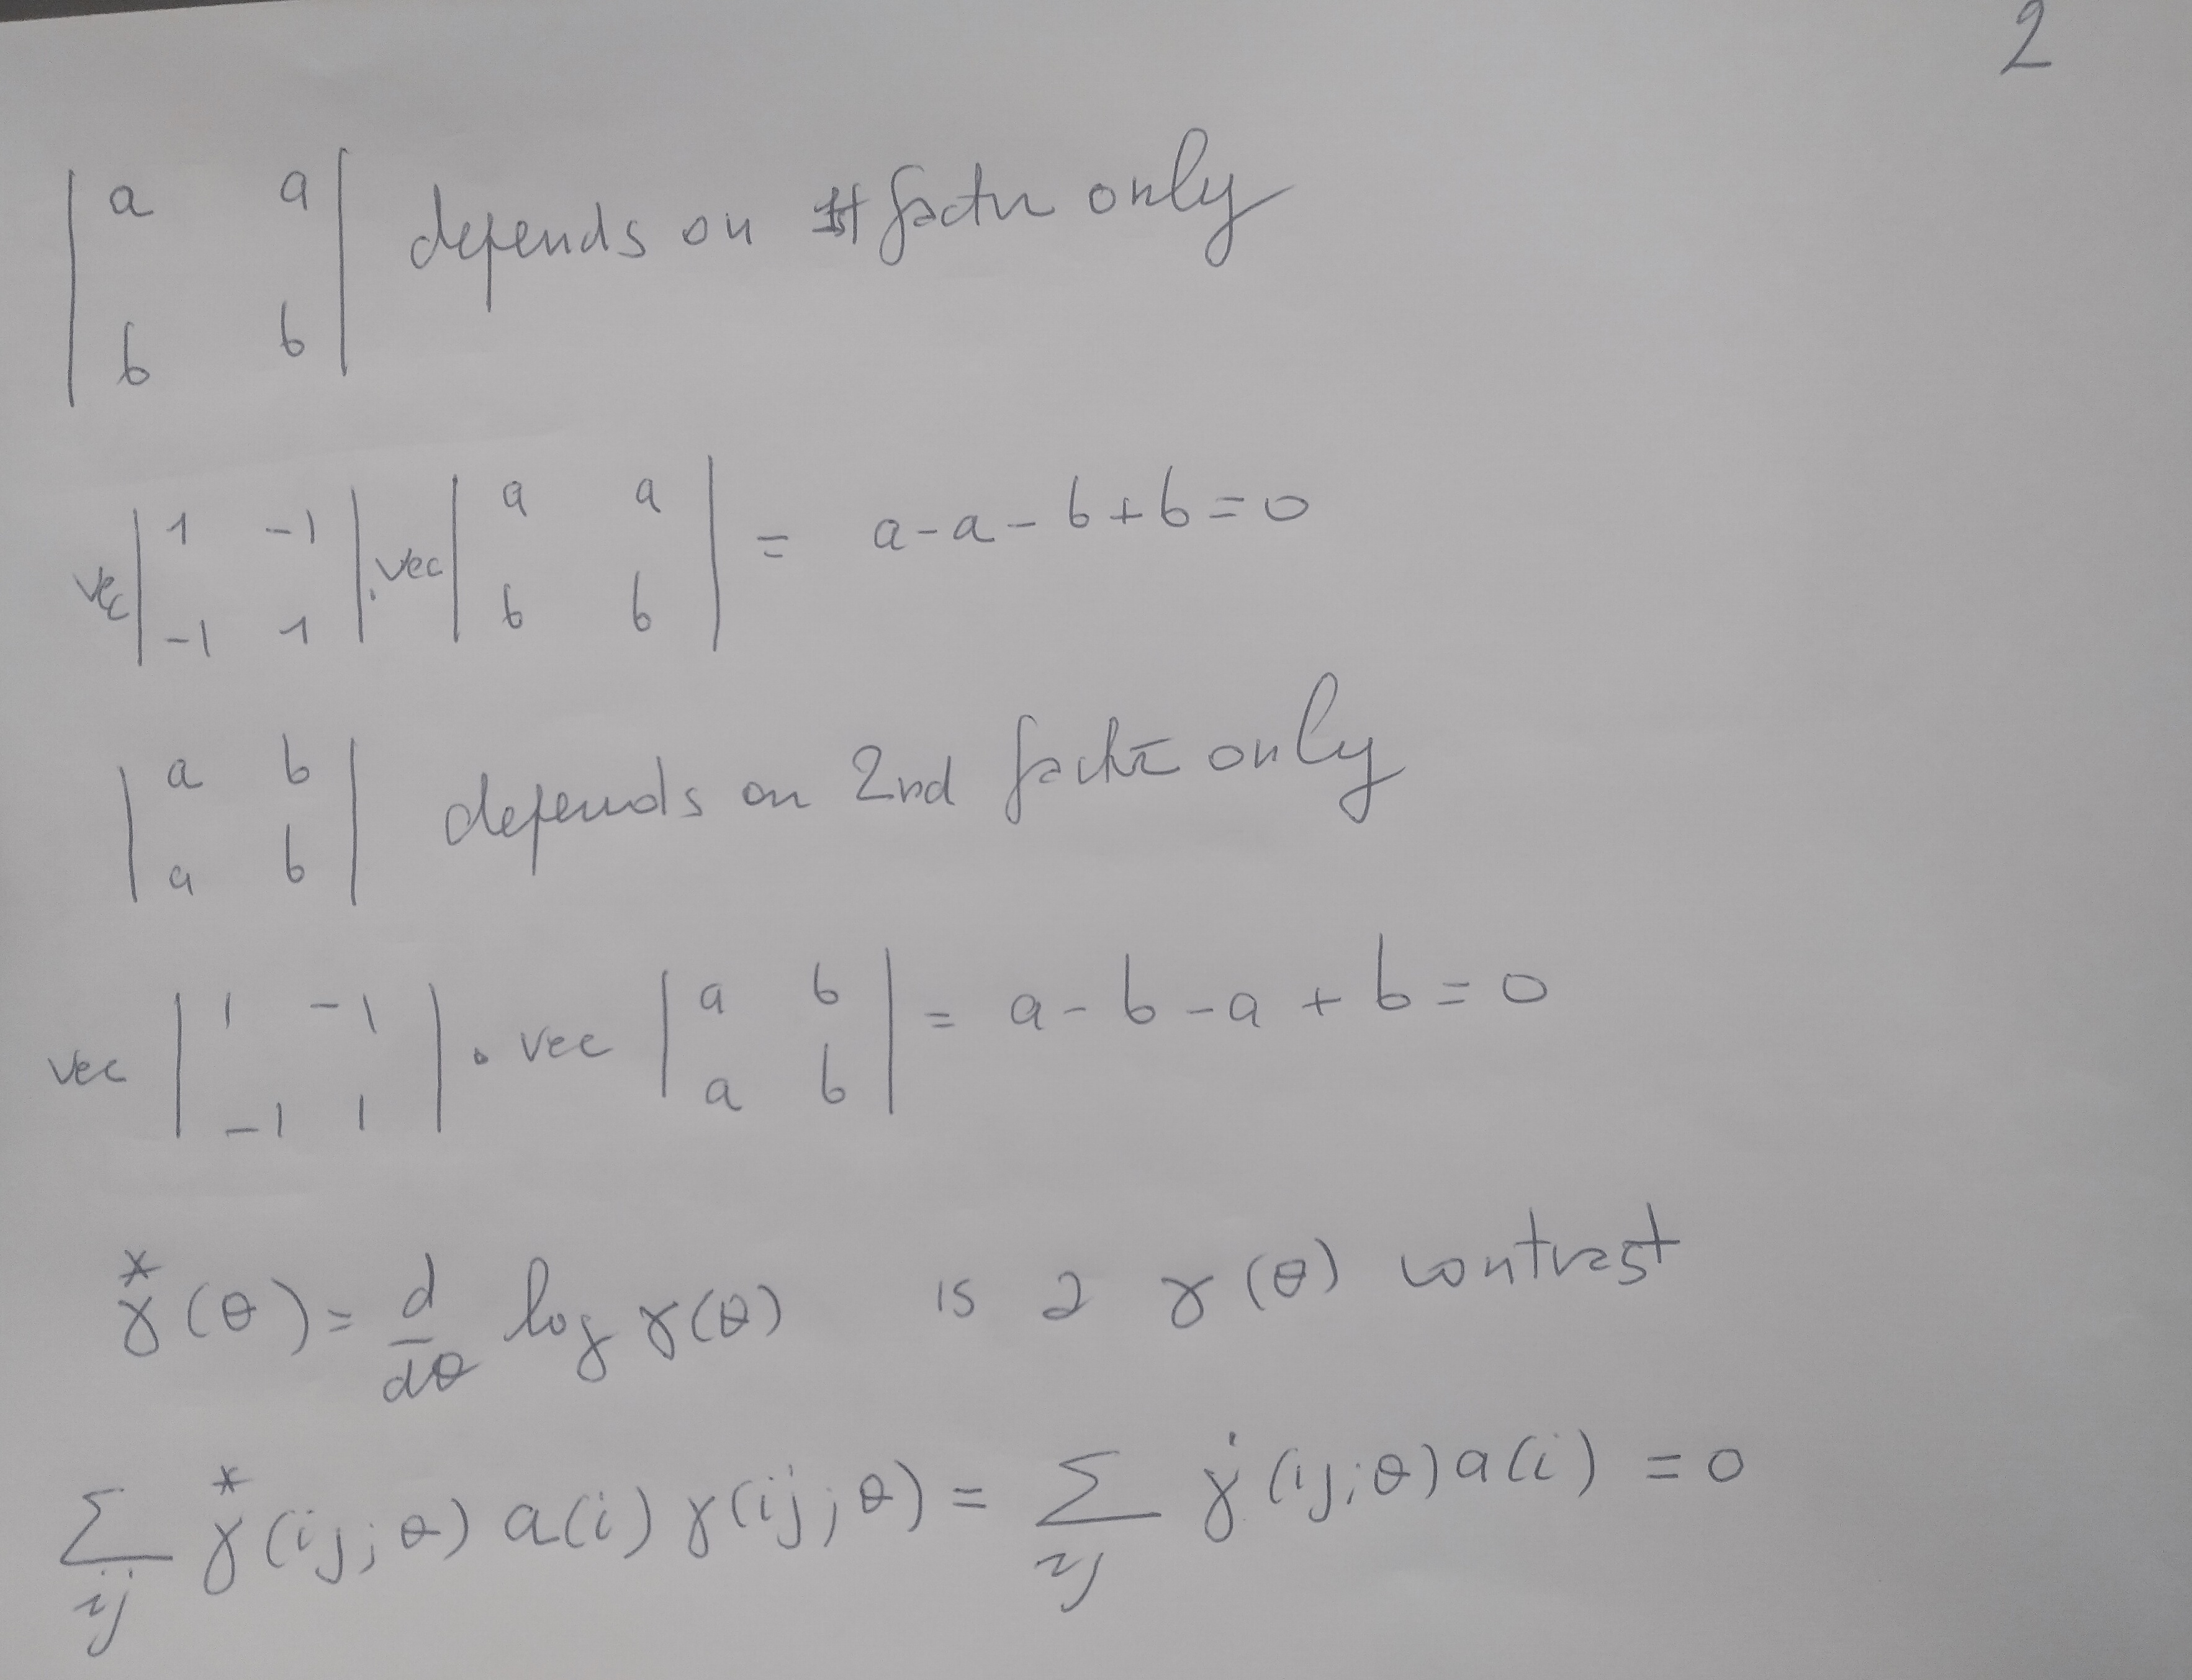
\includegraphics[width=\textwidth]{exercise/2x2-coupling-2.jpg}
    
\end{frame}

\end{document}

%%% Local Variables:
%%% reftex-default-bibliography: ("/home/giannidiorestino/Dropbox/InProgress/tutto.bib")
%%% TeX-master: t
%%% End:

https://www.overleaf.com/project/64109af0a2c0904d6c5e12e8
